\documentclass[border=6pt]{standalone}
\usepackage{tikz}
\usepackage{amsmath}
\usetikzlibrary{positioning,arrows.meta,fit,calc,backgrounds,shapes.geometric}

% New brand ImperialBlue (from ic_eee_thesis.cls)
\definecolor{ImperialBlue}{RGB}{0,0,205}
\definecolor{V2accent}{RGB}{200,80,0}     % orange accent for the V2 guardrail

\begin{document}
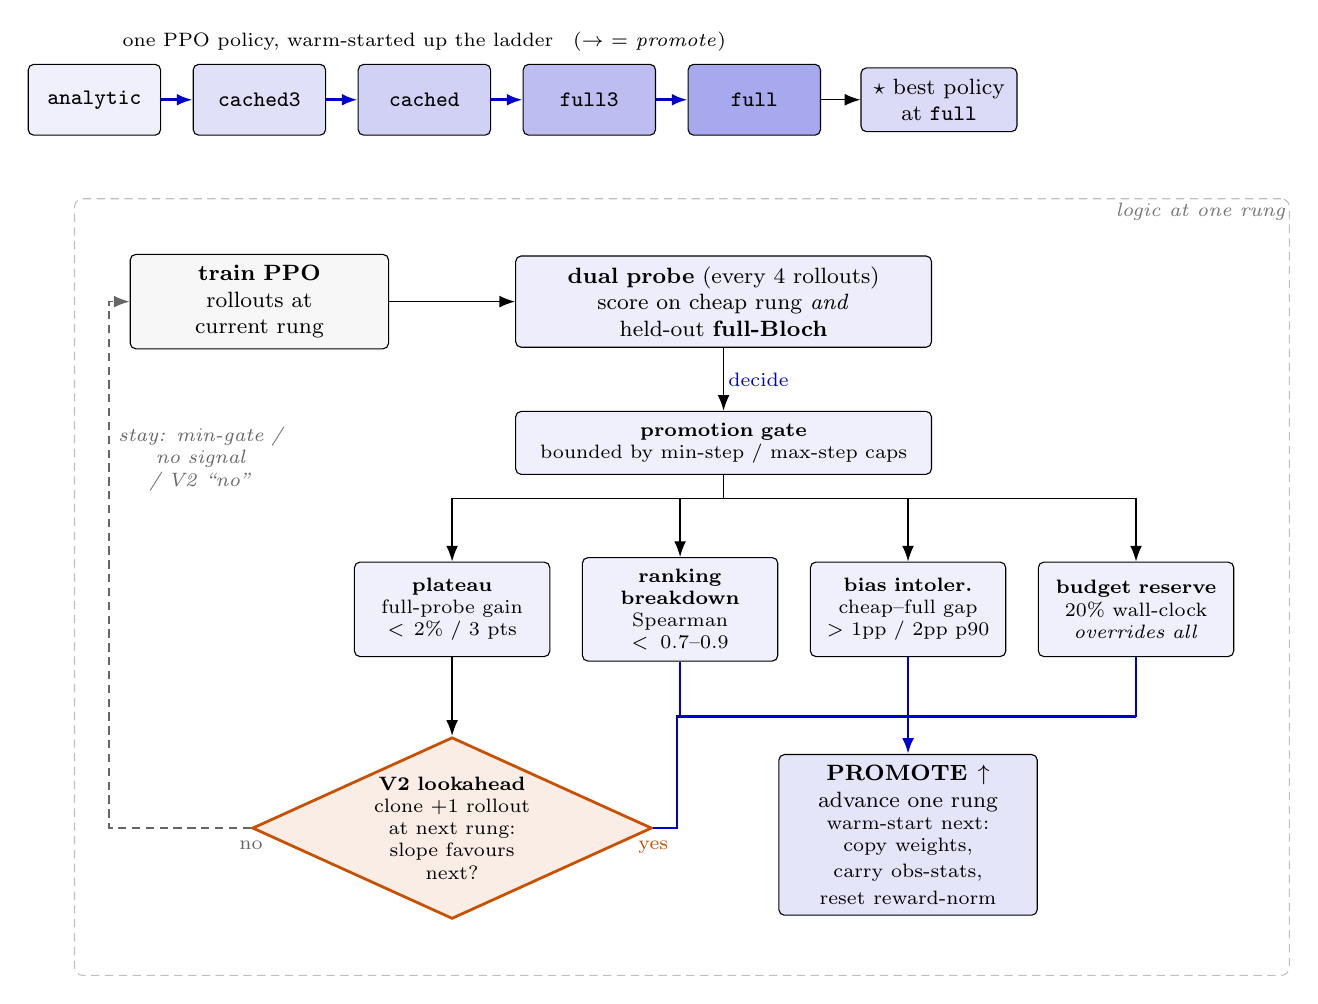
\begin{tikzpicture}[
  font=\footnotesize,
  >={Latex[length=2mm]},
  box/.style={draw, rounded corners=2pt, align=center, inner sep=4pt, minimum height=8mm},
  rung/.style={box, text width=14mm, minimum height=9mm, font=\ttfamily\footnotesize},
  proc/.style={box, fill=black!3, text width=30mm},
  probe/.style={box, fill=ImperialBlue!7, text width=50mm},
  sig/.style={box, fill=ImperialBlue!6, text width=22mm, font=\scriptsize, minimum height=12mm},
  v2/.style={draw=V2accent, line width=1pt, fill=V2accent!10, diamond, aspect=2.2,
             align=center, inner sep=1pt, font=\scriptsize, text width=20mm},
  gate/.style={box, fill=ImperialBlue!6, text width=50mm, font=\scriptsize},
  arr/.style={->, line width=0.5pt},
  promote/.style={->, line width=1pt, ImperialBlue},      % directed (with head)
  promoteline/.style={line width=1pt, ImperialBlue},      % joining segment (no head)
  stay/.style={->, line width=0.6pt, densely dashed, black!60},
  lbl/.style={font=\scriptsize, inner sep=1.5pt},
  plbl/.style={font=\scriptsize, inner sep=1.5pt, ImperialBlue},
]

% ============ LADDER SPINE (top) ============
\node[rung, fill=ImperialBlue!6]  (r1) {analytic};
\node[rung, right=4mm of r1, fill=ImperialBlue!12] (r2) {cached3};
\node[rung, right=4mm of r2, fill=ImperialBlue!18] (r3) {cached};
\node[rung, right=4mm of r3, fill=ImperialBlue!26] (r4) {full3};
\node[rung, right=4mm of r4, fill=ImperialBlue!34] (r5) {full};
\node[box, right=5mm of r5, fill=ImperialBlue!14, text width=17mm, font=\footnotesize]
      (star) {$\star$ best policy\\ at \texttt{full}};
\draw[promote] (r1)--(r2);
\draw[promote] (r2)--(r3);
\draw[promote] (r3)--(r4);
\draw[promote] (r4)--(r5);
\draw[arr] (r5)--(star);
\node[lbl, above=1mm of r3.north] {one PPO policy, warm-started up the ladder \;\;($\rightarrow$ = \textit{promote})};

% ============ INNER LOOP (logic at the current rung) ============
\node[proc, below=15mm of r2.south] (train) {\textbf{train PPO}\\ rollouts at current rung};
\node[probe, right=16mm of train] (probe)
   {\textbf{dual probe} (every 4 rollouts)\\ score on cheap rung \emph{and}\\ held-out \textbf{full-Bloch}};
\draw[arr] (train) -- (probe);

% Gate band
\node[gate, below=8mm of probe] (gate)
   {\textbf{promotion gate}\\ \scriptsize bounded by min-step / max-step caps};
\draw[arr] (probe) -- (gate)
      node[plbl, midway, right] {decide};

% the four signals (any one fires => promote); plateau routes through V2
\node[sig, below left=11mm and 22mm of gate.south] (plateau) {\textbf{plateau}\\ full-probe gain\\ $<2\%$ / 3 pts};
\node[sig, right=4mm of plateau] (rank)    {\textbf{ranking}\\ \textbf{breakdown}\\ Spearman $<0.7$--$0.9$};
\node[sig, right=4mm of rank]    (bias)    {\textbf{bias intoler.}\\ cheap--full gap\\ $>1$pp / $2$pp p90};
\node[sig, right=4mm of bias]    (budget)  {\textbf{budget reserve}\\ 20\% wall-clock\\ \emph{overrides all}};
\draw[arr] (gate.south) -- ++(0,-3mm) -| (plateau.north);
\draw[arr] (gate.south) -- ++(0,-3mm) -| (rank.north);
\draw[arr] (gate.south) -- ++(0,-3mm) -| (bias.north);
\draw[arr] (gate.south) -- ++(0,-3mm) -| (budget.north);

% V2 lookahead decision on the plateau branch (flagged, co-equal node)
\node[v2, below=10mm of plateau, xshift=0mm] (v2)
     {\textbf{V2 lookahead}\\ clone $+1$ rollout\\ at next rung:\\ slope favours next?};
\draw[arr] (plateau) -- (v2);

% ---- collector bus: one arrowhead total (into PROMOTE) ----
\coordinate (busy) at ($(rank.south)+(0,-7mm)$);
% direct signals drop onto the bus (no heads)
\draw[promoteline] (rank.south)   -- (rank.south   |- busy);
\draw[promoteline] (bias.south)   -- (bias.south   |- busy);
\draw[promoteline] (budget.south) -- (budget.south |- busy);
% V2 "yes" joins from the right (no head)
\draw[promoteline] (v2.east) -- ++(3mm,0) |- (bias.south |- busy);
\node[plbl, V2accent, below=3pt of v2.east] {yes};
% horizontal bus
\draw[promoteline] (rank.south |- busy) -- (budget.south |- busy);
% single directed exit into PROMOTE
\coordinate (sigmid) at ($(rank.south)!0.5!(budget.south)$);
\node[box, fill=ImperialBlue!10, text width=30mm, font=\footnotesize]
     (promoteout) at ($(sigmid |- busy) + (0,-15mm)$)
     {\textbf{PROMOTE}\;\,$\uparrow$ advance one rung\\ \scriptsize warm-start next: copy weights,\\ carry obs-stats, reset reward-norm};
\draw[promote] (sigmid |- busy) -- (promoteout.north);

% V2 "no" exits LEFT -> short left-gutter stay loop back to train
\draw[stay] (v2.west) -- ++(-18mm,0) |- (train.west);
\node[lbl, black!60, below=3pt of v2.west] {no};
\node[lbl, black!60, anchor=center, align=center, text width=22mm]
      at ($(train.west)+(+9mm,-20mm)$)
      {\itshape stay: min-gate /\\ no signal / V2 ``no''};

% dashed enclosure to mark "the logic at one rung"
\begin{scope}[on background layer]
\node[draw=black!25, densely dashed, rounded corners=3pt, inner sep=7mm,
      fit=(train)(probe)(gate)(plateau)(budget)(v2)(promoteout)] (loopbox) {};
\end{scope}
\node[lbl, anchor=north east, black!55] at (loopbox.north east) {\itshape logic at one rung};

\end{tikzpicture}
\end{document}
